\section{DROP: Workload Optimization}
\label{sec:algo}


We now introduce DROP, a system that performs progressive sampling and online progress estimation to control the amount of sampling to minimize overall runtime. 
DROP answers a crucial question that stochastic PCA techniques have traditionally ignored: how long should these methods run? 

\begin{comment}
Notation used is in Table~\ref{table:inputs}.

\begin{table}
\centering
\small
\caption{\label{table:inputs} 
 DROP algorithm notation and defaults}
{\renewcommand{\arraystretch}{1.2}
\begin{tabular}{|c|l l|}
\hline 
Symbol & Description (\emph{Default}) & Type\tabularnewline
\hline
$X$  & Input dataset                          & $\mathbb{R}^{\mvar \times \dvar}$ \tabularnewline
$\mvar$  & Number of input data points            & $\mathbb{Z}_{+}$\tabularnewline
$\dvar$  & Input data dimension                   & $\mathbb{Z}_{+}$ \tabularnewline
$B$  & Target $TLB$ preservation      		 & $0 < \mathbb{R} \leq 1 $ \tabularnewline
$\mathcal{C}_\mvar(\dvar)$  & Downstream runtime function (\textit{k-NN runtime})       & $\mathbb{Z}_{+} \to \mathbb{R}_{+}$\tabularnewline
$R$  & Total DROP runtime       & $\mathbb{R}_{+}$ \tabularnewline
$c$ & Confidence level for $TLB$ preservation (\textit{$95 \%$})          & $\mathbb{R}$  \tabularnewline
$T_k$  & DROP output $k$-dimensional transformation &$\mathbb{R}^{\dvar \times k}$ \tabularnewline
$i $ & Current DROP iteration        & $\mathbb{Z}_+$  \tabularnewline

\hline 
\end{tabular}
}
\end{table}
\end{comment}

\begin{figure*}
\label{fig:arch}
\begin{center}
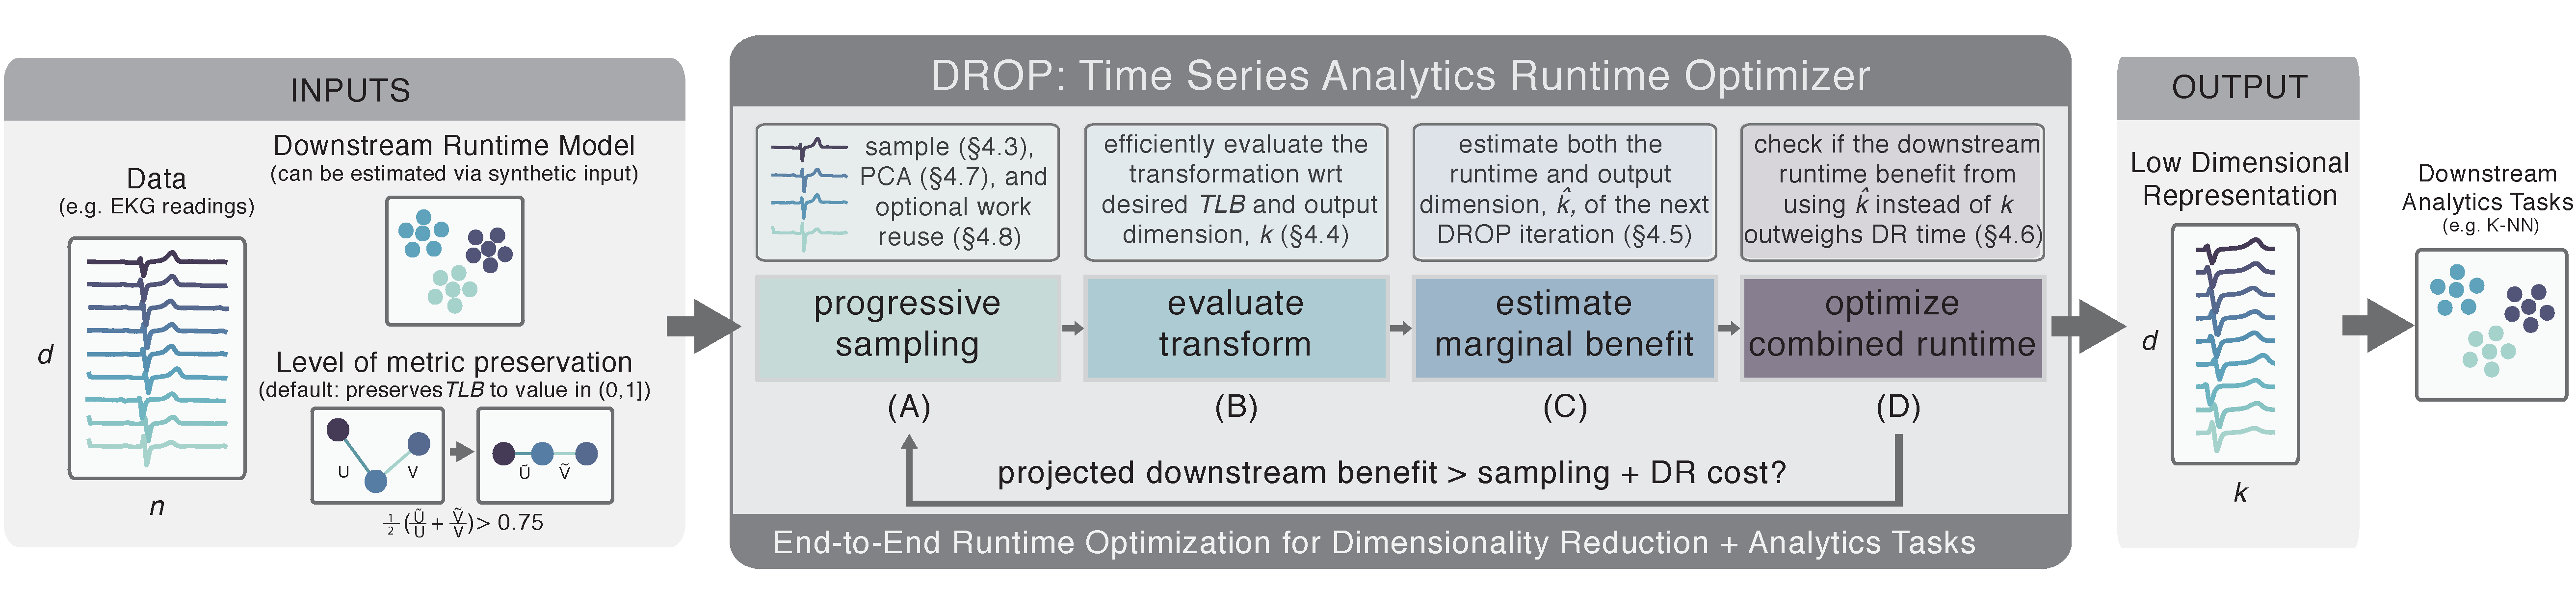
\includegraphics[width=\textwidth]{figs/system_arch.pdf}\vspace{-1em}
\caption[]{High-level DROP architecture depicting DROP's inputs, outputs, and core components.}
\end{center}
\vspace{-1em}
\end{figure*}


\subsection{DROP Architecture}
\label{subsec:arch}
%DROP is a system that performs workload-aware dimensionality reduction, optimizing the combined runtime of downstream tasks and DR as defined in Problem~\ref{def:opt}.
DROP operates over a series of progressively larger data samples, and determines when to terminate via \red{a} four-step procedure that is repeated for each iteration: progressive sampling, transformation evaluation, progress estimation, and cost-based optimization:
%To power this pipeline, DROP combines database and machine learning techniques spanning online aggregation (\S\ref{subsec:teval}), progress estimation (\S\ref{subsec:pest}), progressive sampling (\S\ref{subsec:psample}), and PCA approximation (\S\S\ref{subsec:pcaroutine},\ref{subsec:reuse}).

%We now provide a brief overview of DROP's sample-based iterative architecture before detailing each.


\minihead{Step 1: Progressive Sampling (\S\ref{subsec:psample}, Alg~\ref{alg:DROP} L\ref{eq:sample}, Fig 2A)}

\noindent DROP draws a data sample and performs PCA over this sample. Additionally, DROP makes use of a novel means of reusing work across iterations (\S\ref{subsec:reuse}).

\minihead{Step 2: Transform Evaluation (\S\ref{subsec:teval}, Alg~\ref{alg:DROP} L\ref{eq:evaluate}, Fig 2B)} 

\noindent Given the PCA result from Step 1, DROP evaluates its quality by identifying the size of the smallest metric-preserving transformation that can be extracted. 

\minihead{Step 3: Progress Estimation (\S\ref{subsec:pest}, Alg~\ref{alg:DROP} L\ref{eq:estimate}, Fig 2C)} 

\noindent Given the size of the metric-preserving transform and the computation time required to obtain this transform, DROP estimates the size and computation time of running an additional DROP iteration.

\minihead{Step 4: Cost-Based Optimization (\S\ref{subsec:opt}, Alg~\ref{alg:DROP} L\ref{eq:optimize}, Fig 2D)} 

\noindent Given this and the estimated future iteration's transformation sizes and computation times, DROP optimizes over the end-to-end DR and downstream task runtime to determine if it should terminate.

\subsection{Progressive Sampling}
\label{subsec:psample}
DROP repeatedly chooses a subset of data and computes PCA on the subsample (via one of several methods described in Section~\ref{subsec:pcaroutine}).
By default, we consider a simple uniform sampling strategy where at each iteration, DROP samples a fixed percentage of the data.
Exploring data-dependent and weighted sampling schemes that are dependent on the current basis is an exciting area for future work. 
%While we considered a range of alternative sampling strategies, uniform sampling strikes a balance between computational and statistical efficiency. 
%Data-dependent and weighted sampling schemes that are dependent on the current basis may decrease the total number of iterations required by DROP, but may require expensive reshuffling of data at each iteration~\cite{coresets}. 

%DROP provides configurable strategies for both base number of samples and the per-iteration increment, in our experimental evaluation in Section~\ref{sec:experiments}, we consider a sampling rate of $1\%$ per iteration.
%We discuss more sophisticated additions to this base sampling schedule in the extended manuscript.

\begin{algorithm}[t!]
\begin{algorithmic}[1]
\small
\Statex \textbf{Input:}  
\Statex $X$: data matrix
\Statex $B$: target metric preservation level
\Statex $\mathcal{C}_\mvar$: cost of downstream operations; default tuned to k-NN
\Statex
\Statex \textbf{Output:}   
\Statex $T_k$: $k$-dimensional transformation matrix
\Statex
\Statex \hrule
\Function{drop}{$X,  B, \mathcal{C}_\mvar$}:
	\State Initialize: $i = 0; k_0 = \infty$ 
		\Comment{iteration and current basis size}
	\Do
		\State i$\texttt{++}$, \textsc{clock.restart}
		\State $X_i$ = \textsc{sample}($X, \textsc{sample-schedule}(i)$) \label{eq:sample}
			\Comment{\S~\ref{subsec:psample}}
		\State $T_{k_i}$ = \textsc{compute-transform}($X, X_i,  B$) \label{eq:evaluate}
			\Comment{\S~\ref{subsec:teval}}
		\State $r_i = \textsc{clock.elapsed}$	
			\Comment{$R = \sum_i r_i$}
		\State $\hat{k}_{i+1}, \hat{r}_{i+1} $ = \textsc{estimate}($k_i, r_i$) \label{eq:estimate}
			\Comment{\S~\ref{subsec:pest}}
	\doWhile{\textsc{optimize}($\mathcal{C}_\mvar,k_i,r_i,\hat{k}_{i+1}, \hat{r}_{i+1}$)} \label{eq:optimize}
		\Comment{\S~\ref{subsec:opt}}
	\\\Return{$T_{k_i}$}
\EndFunction
\end{algorithmic}
\caption{DROP Algorithm}
\label{alg:DROP}
\end{algorithm}



\subsection{Evaluating Transformations}
\label{subsec:teval}
Given a transformation obtained by running PCA over a sample, DROP must accurately and efficiently evaluate the performance of this transformation with respect to a metric of interest \red{over the entire dataset, not just the data sample}. 
%To do so, DROP adapts an approach for deterministic queries in online aggregation: treating quality metrics as aggregation functions and using confidence intervals for fast estimation. 
%We first discuss this approach in the context of $TLB$, then discuss how to extend this approach to alternative metrics at the end of this section.

We define the performance of a transformation computed over a sample as the size of the lowest dimensional $TLB$-preserving transform that can be extracted.
There are two challenges in evaluating this performance, which DROP overcomes.
First, the size of the lowest dimensional transformation that achieves $TLB$ constraints is rarely known a priori. 
Second, brute-force $TLB$ computation would dominate the runtime of computing PCA over a sample.

\subsubsection{Computing the Lowest Dimensional Transformation}


DROP first computes a full, $\dvar$-dimensional basis (i.e., of dimension equal to the input dimension) via PCA over the data sample.
To reduce dimensionality, DROP must determine if a smaller dimensional $TLB$-preserving transformation can be computed over this sample, and return the smallest such transform. 
Ideally, the dimension of the best (smallest) transformation would be known, but in practice, this information is rarely known a priori.   
Therefore, DROP uses the $TLB$ constraint to automatically identify the size of the returned transformation.
A na\"ive strategy would evaluate the $TLB$ for every combination of the $\dvar$ basis vectors for every transformation size, requiring $O(2^\dvar)$ evaluations. 
Instead, DROP exploits two key properties of PCA to avoid this.

First, PCA via SVD produces an orthogonal linear transformation where the first principal component explains the most variance in the dataset, the second explains the second most---subject to being orthogonal to the first---and so on.  
Therefore, once DROP has computed the transformation matrix for dimension $\dvar$, DROP obtains the transformations for all dimensions $k$ less than $\dvar$ truncating the matrix to dimension $\dvar \times k$.

Second, with respect to $TLB$ preservation, the more principal components that are retained, the better the lower-dimensional representation in terms of $TLB$.  
This is because orthogonal transformations such as PCA preserve inner products. 
Therefore, a full PCA (where no dimensions are omitted) perfectly preserves $\mathcal{L}_2$-distance between data points. 
As the $\mathcal{L}_2$-distance is a sum of squared (positive) terms, the more principal components that are retained, the better the representation preserves $\mathcal{L}_2$-distance.

Using the first property (i.e., PCA's ordering), DROP obtains all low-dimensional transformations for the sample from the $\dvar$-dimensional basis.  
Using the second property (i.e., of monotonicity of principal components), DROP then runs binary search over these transformations to find and return the lowest-dimensional basis that attains $B$ (i.e., \textsc{compute-transform}, line~\ref{eq:basis} of Algorithm~\ref{alg:candidate}).
If a target $B$ cannot be realized with this sample, DROP omits all further optimization steps in this iteration and continues the next iteration by drawing a larger sample.

Computing the full $\dvar$-dimensional basis at every step may be wasteful. 
To avoid this need, DROP's exploits information from previous iterations:  if DROP has previously found a candidate $TLB$-preserving basis of size $\dvar' < \dvar$ in prior iterations, then DROP only computes $\dvar'$ components at the start of the next iteration. \red{This is because similar to a hold-out or validation set, $TLB$ evaluation is representative of the entire dataset, not just the current sample (see Alg.~\ref{alg:candidate} L5). 
Thus, sampling additional training datapoints enables DROP to better learn global data structure and perform at least as well as over a smaller sample.}
This reduces the space of lower dimensions to consider, and allows for more efficient PCA computation for future iterations, as advanced PCA routines can exploit the $\dvar'$-th eigengap to converge faster (\S\ref{sec:relatedwork}).

% stop here!

\subsubsection{$TLB$ Computation}

Given a transformation, DROP must efficiently determine if the basis preserves the desired $TLB$.
Computing pairwise $TLB$ for all data points requires $O(\mvar^2\dvar)$ time, which dominates the runtime of computing PCA on a sample.
However, as the $TLB$ is an average of random variables bounded from 0 to 1, DROP can adapt techniques from online aggregation and approximate query processing~\cite{onlineagg,barzan-keynote}, using statistical sampling and confidence intervals to compute the $TLB$ to arbitrary confidences.

Given a transformation, DROP iteratively refines an estimate of its $TLB$ (function \textsc{evaluate-tlb} in Algorithm~\ref{alg:candidate}, line~\ref{eq:eval}) by \red{incrementally sampling an increasing number of} pairs from the input data (Algorithm~\ref{alg:candidate}, line~\ref{eq:paircheck}), transforming each pair into the new basis, then measuring the distortion of $\mathcal{L}_2$ distance between the pairs, providing a $TLB$ estimate to confidence level $c$ (Algorithm~\ref{alg:candidate}, line~\ref{eq:tlbeval}). 
If the confidence interval's lower bound is greater than the target $TLB$, the basis is a sufficiently good fit; if its the upper bound is less than the target $TLB$, the basis is not a sufficiently good fit. 
If the confidence interval contains the target $TLB$,  \red{ DROP is unable to conclude whether or not the target $TLB$ is achieved. Thus, DROP automatically samples additional pairs to refine its estimate; in practice, and especially for our initial target time series datasets, DROP rarely uses more than 500 pairs on average in its $TLB$ estimates (often using far fewer)}.

To estimate the $TLB$ to confidence $c$, DROP uses the Central Limit Theorem (similar to online aggregation~\cite{onlineagg}): computing the standard deviation of a set of sampled pairs' $TLB$ measures and applying a confidence interval to the sample according to the $c$.
For data with low variance, DROP evaluates a candidate basis with few samples from the dataset \red{as the confidence intervals shrink rapidly}. 

The techniques in this section are presented in the context of $TLB$, but can be applied to any downstream task and metric for which we can compute confidence intervals and are monotonic in number of principal components retained.
\red{For instance, DROP can operate while using all of its optimizations when using any $L^p$-norm.}
\red{Euclidean similarity search} is simply one such domain that is a good fit for PCA: when performing DR via PCA, as we increase the number of principal components, a clear positive correlation exists between the percent of variance explained and the $TLB$ regardless of data spectrum.
We demonstrate this correlation in the experiment below, where we generate three synthetic datasets with predefined spectrum (right), representing varying levels of structure present in real-world datasets. 
The positive correlation is evident (left) despite the fact that the two do not directly correspond ($x=y$ provided as reference). 
This holds true for all of the evaluated real world datasets.

\vspace{.2cm}
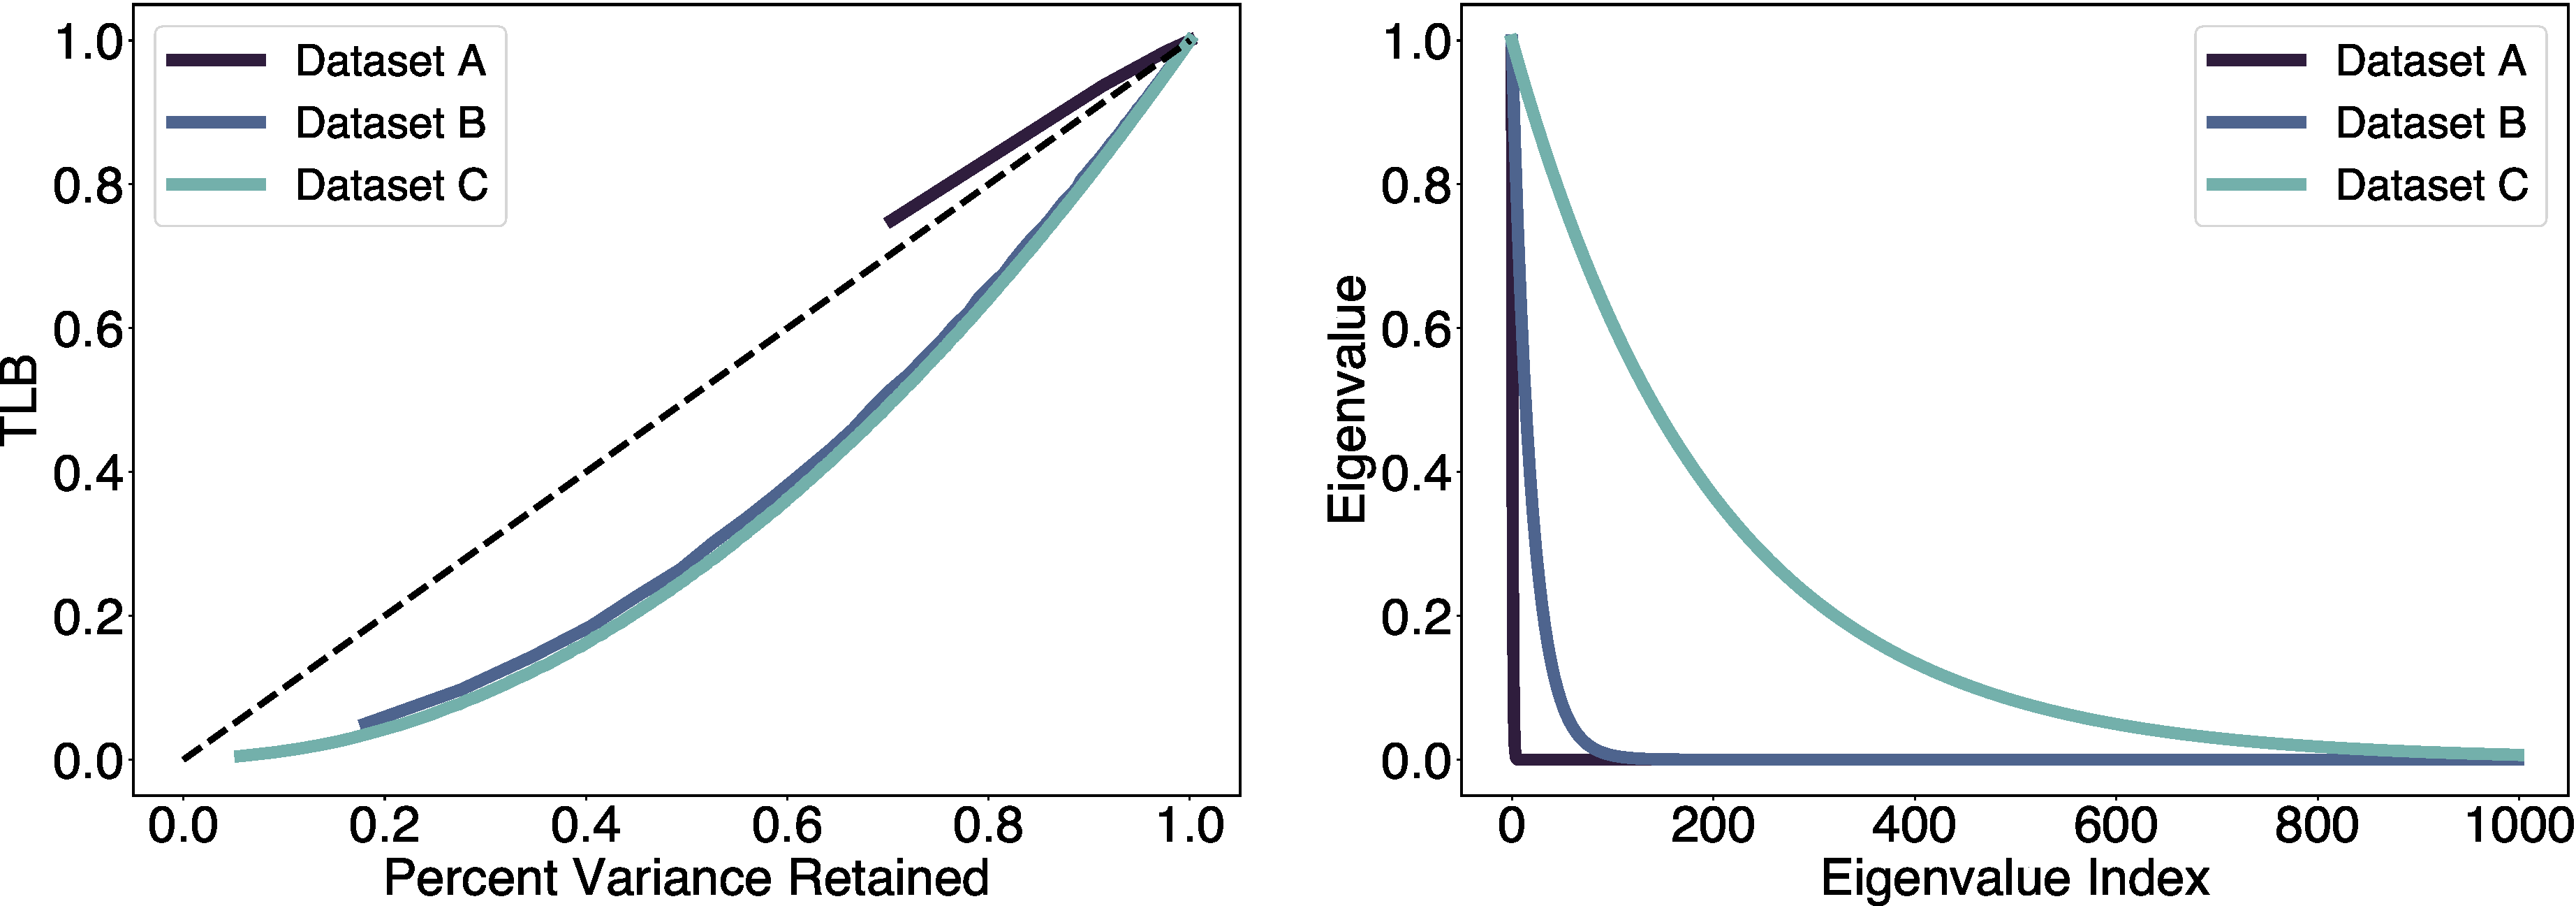
\includegraphics[width= .9\linewidth]{figs/tlb-pca.pdf}

For alternative preservation metrics, we can utilize closed-form confidence intervals~\cite{stats-book,ci1,onlineagg}, or bootstrap-based methods~\cite{bootstrap1,bootstrap2}, which incur higher overhead but can be more generally applied.


\begin{algorithm}
\begin{algorithmic}[1]
\small
\Statex \textbf{Input:}  
\Statex $X$: sampled data matrix
\Statex $B$: target metric preservation level; default $TLB = 0.98$
\Statex  \hrule 
\Function{compute-transform}{$X, X_i B$}: \label{eq:basis}
	\State \textsc{pca.fit}$(X_i)$
			\Comment{fit PCA on the sample}
	\State Initialize: high $= k_{i-1}$; low $=0$; $k_i= \frac{1}{2}$(low + high); $B_i = 0$
	\While{(low $!=$ high)}
		\State $T_{k_i}, B_i  = \textsc{evaluate-tlb}( X, B, k_i)$
		\If{$B_i \leq B$}  low $= k_i + 1$ 
		\Else  \hspace{0pt} high $= k_i $
		\EndIf
		\State $k_i = \frac{1}{2}$(low + high)
	\EndWhile
	\State $T_{k_i} = $ cached $k_i$-dimensional PCA transform\\
	\Return $T_{k_i}$
\EndFunction
\Statex 
\Function{evaluate-tlb}{$X, B, k$}: \label{eq:eval}
	\State numPairs $= \frac{1}{2}\mvar(\mvar-1)$
	\State $p = 100$
		\Comment{number of pairs to check metric preservation}
	\While{($p < $ numPairs)}
		\State $B_i, B_{lo}, B_{hi} = $ \textsc{tlb}($ X, p, k$)
			 \label{eq:paircheck}
		\If{($B_{lo} > B$ or $B_{hi} < B$)}   \textbf{break}
		\Else \hspace{0pt} pairs $\times$= $ 2$
		\EndIf
	\EndWhile
	\\\Return $B_i$	
\EndFunction
\Statex 
\Function{tlb}{$X, p, k$}: \label{eq:tlbeval}
	\State \textbf{return } mean and 95\%-CI of the $TLB$ after transforming $p$ $d$-dimensional pairs of points from $X$ to dimension $k$. The highest transformation computed thus far is cached to avoid recomputation of the transformation matrix.
\EndFunction

\end{algorithmic}
\caption{Basis Evaluation and Search}
\label{alg:candidate}
\end{algorithm}


\subsection{Progress Estimation}
\label{subsec:pest}
Given a low dimensional $TLB$-achieving transformation from the evaluation step, DROP must identify the quality (dimensionality) and cost (runtime) of the transformation that would be obtained from an additional DROP iteration.
%We refer to this as the $progress estimation$ step.

Recall that DROP seeks to minimize objective function $R + \mathcal{C}_\mvar(k)$ such that $TLB(XT_k) \geq B$, with $R$ denoting DROP's total runtime, $T_k$ the $k$-dimensional $TLB$-preserving transformation of data $X$ returned by DROP, and $\mathcal{C}_\mvar(k)$ the workload cost function. 
Therefore, given a $k_i$-dimensional transformation $T_{k_i}$ returned by the evaluation step of DROP's $i^{\text{th}}$ iteration, DROP can compute the value of this objective function by substituting its elapsed runtime for $R$ and $T_{k_i}$ for $T_k$.  
We denote the value of the objective at the end of iteration $i$ as $obj_i$. 
To decide whether to continue iterating to find an improved transformation, DROP must be able to estimate the objective function value of future iterations.

In Section~\ref{subsec:opt} we show that DROP requires $obj_{i+1}$ to minimize this objective function.
To estimate $obj_{i+1}$, DROP must estimate the runtime required for iteration $i+1$ (which we denote as $r_{i+1}$, where $R=\sum_i r_i$ after $i$ iterations) and the dimensionality of the $TLB$-preserving transformation produced by iteration $i+1$, $k_{i+1}$. 
Because DROP cannot directly measure $r_{i+1}$ or $k_{i+1}$ without performing iteration $i+1$, DROP performs online progress estimation to estimate these quantities. Specifically, DROP performs online parametric fitting to compute future values based on prior values for $r_{i}$ and $k_i$ in line~\ref{eq:estimate} of Algorithm~\ref{alg:DROP}. 
By default, given a sample of size $m_i$ in iteration $i$, DROP performs linear extrapolation to estimate $k_{i+1}$ and $r_{i+1}$. The estimate of $r_{i+1}$, for instance, is:

\vspace{-.4cm}
\begin{equation*}
\hat{r}_{i+1} = r_i + \frac{r_i - r_{i-1}}{m_i - m_{i-1}} (m_{i+1} -  m_i)
\end{equation*}


\red{
DROP's use of a basic first-order approximation is motivated by the fact that when adding a small number of data samples each iteration, both runtime and resulting lower dimension do not change drastically (i.e., see Fig.~\ref{fig:progressive} after a feasible point is achieved). 
While linear extrapolation acts as a proof-of-concept for progress estimation, the architecture can incorporate more sophisticated functions as needed (\S\ref{sec:relwork}).
}

\subsection{Cost-Based Optimization}
\label{subsec:opt}

Given the results of the progress estimation step, DROP must determine if continued PCA on additional samples will be beneficial to overall runtime, or if it is better to terminate. 
%We refer to this as the $cost-based optimization$ step. 

Given predictions of the next iteration's runtime ($\hat{r}_{i+1}$) and dimensionality ($\hat{k}_{i+1}$), DROP uses a greedy heuristic in estimating the optimal objective-minimizing stopping point.
Concretely, if the objective function estimate for the next iteration is greater than its current objective function value ($obj_i < \widehat{obj}_{i+1}$), then DROP will terminate. 
If DROP's runtime is convex in the number of iterations, it is straightforward to prove that this condition is in fact the optimal stopping criterion (i.e., via convexity of composition of convex functions). 
This stopping criterion leads to a simple check at each DROP iteration that is used by  \textsc{optimize} in Algorithm~\ref{alg:DROP} line~\ref{eq:optimize}: 

\vspace{-.4cm}
\begin{align}
  obj_i &< \widehat{obj}_{i+1} \nonumber \\
  \mathcal{C}_\mvar(k_i) + \sum_{j=0}^i r_j &< \mathcal{C}_\mvar(\hat{k}_{i+1}) + \sum_{j=0}^{i} r_j + \hat{r}_{i+1} \nonumber \\
  % \mathcal{C}_\mvar(k_i)  &< \mathcal{C}_\mvar(\hat{k}_{i+1}) + \hat{r}_{i+1}  \nonumber \\
  \mathcal{C}_\mvar(k_i) - \mathcal{C}_\mvar(\hat{k}_{i+1}) &< \hat{r}_{i+1}  \label{eq:check}
\end{align}

DROP terminates when the projected time of the next iteration exceeds the estimated downstream runtime benefit. 

\red{While we empirically observed the runtime to be convex, this does not hold true in the general case as the rate of decrease in dimension ($k_i$) is data dependent. 
Should $k_i$ plateau before continued decrease, DROP will terminate prematurely. 
We encounter this scenario during DROP's first iterations if sufficient data to meet the $TLB$ threshold at a dimension lower than $\dvar$ had not been sampled (SmallKitchenAppliances in Fig.~\ref{fig:progressive}).
To combat this challenge, optimization is only enabled once a feasible point is attained as we prioritize accuracy over runtime (i.e., $0.3$ for SmallKitchenAppliances in Fig.~\ref{fig:progressive}).
We show the implications of this decision in DROP in Section~\ref{subsec:lesion}.%, and in the streaming setting in the extended manuscript.
}

\subsection{Choice of PCA Subroutine}
\label{subsec:pcaroutine}

At each iteration, DROP uses PCA as its means of DR.
The most straightforward means of implementing this PCA step is to compute a full SVD over the data (\S\ref{sec:pca}).
There are many suitable libraries for this task---many of which are highly optimized---and therefore this strategy is pragmatic and easy to implement. 
However, this approach is computationally inefficient compared to other DR techniques (\S\ref{sec:background}).  

In our DROP implementation, we compute PCA via a randomized SVD algorithm by Halko, Martinsson, and Tropp (SVD-Halko) that calculates an approximate rank-$k$ factorization (truncated SVD) of a data matrix~\cite{tropp}. 
While additional advanced methods for efficient PCA exist (\S\ref{sec:relwork}), we found that not only is SVD-Halko asymptotically of the same running time as techniques used in practice (such as probabilistic PCA used in a recent SIGMOD 2015 paper on scalable PCA~\cite{ppca-sigmod}), it is straightforward to implement, can take advantage of optimized linear algebra libraries, and does not require tuning for hyperparameters such as batch size, learning rate, or convergence criteria.  
SVD-Halko is not as efficient as other techniques with respect to communication complexity, as probabilistic PCA used in~\cite{ppca-sigmod}, or convergence rate, as recent work in accelerated, momentum-based PCA~\cite{re-new}.
However, these techniques can be easily substituted for SVD-Halko in DROP's architecture.
%%%%We demonstrate this by implementing multiple alternatives in Section~\ref{subsec:pcaexp}.
%%%%\red{Further, we also demonstrate that this implementation is competitive with the widely used SciPy Python library~\cite{scipy}}.

\begin{comment}
\begin{algorithm}[t]
\begin{algorithmic}
\State \textbf{Input:}  \\
$H$: concatenation of previous transformation matrices \\
$T$: new sample's transformation \\
 points to sample per iteration; default 5\% \\
 
\\ \hrule

\Function{distill}{$H, T$}:
	\State $H \gets [H | T]$
		\Comment{Horizontal concatenation to update history}
	\State $U, \Sigma, V^\intercal \gets \textsc{SVD}(H)$ 
				\Comment{$U$ is a basis for the range of $T$}
	\State $T \gets U[:,\textsc{num-columns(T)}]$
	\\\Return{$T$}
\EndFunction
\end{algorithmic}
\caption{Work Reuse}
\label{alg:reuse}
\end{algorithm} 
\end{comment}

\subsection{Work Reuse}
\label{subsec:reuse}

A natural question arises due to DROP's iterative architecture: can we combine the information from each sample's transformation without computing PCA over the union of the sampled data points? 
While stochastic methods for PCA enable such work reuse across samples as they iteratively refine a single transformation matrix, other methods do not.
We propose an algorithm that allows reuse of previous work when utilizing arbitrary PCA routines with DROP.

DROP uses two key insights in order to enable this work reuse.  
First, given two transformation matrices produced via PCA, $T_1$ and $T_2$, the horizontal concatenation of these matrices $H = [T_1 | T_2]$ is a transformation into the union of their range spaces.
Second, for datasets that have rapid drop off in spectrum, the principal components returned from running PCA on repeated data samples will generally concentrate to the true top principal components. 
Thus, work reuse proceeds via two step concatenate-distill approach:
DROP first maintains a transformation history consisting of the horizontal concatenation of all PCA transformations to this point, and then computes the SVD of this history matrix and returns the first $k$ columns as the transformation matrix. 

Although this routine requires an SVD computation, computational overhead is not dependent on the raw dataset size, but on the size of the history matrix, $H$.
This size is proportional to the original dimensionality $\dvar$ and size of lower dimensional transformations, which are in turn proportional to the data's intrinsic dimensionality and the $TLB$ constraint.
As preserving \emph{all history} can be expensive in practice, 
DROP periodically shrinks the history matrix using DR via PCA. 
We validate the benefit of using work reuse---up to \red{15\%} on real-world data---in Section~\ref{sec:experiments}.

